\documentclass{article}%
\usepackage[T1]{fontenc}%
\usepackage[utf8]{inputenc}%
\usepackage{lmodern}%
\usepackage{textcomp}%
\usepackage{lastpage}%
\usepackage[head=40pt,margin=0.5in,bottom=0.6in]{geometry}%
\usepackage{graphicx}%
%
\title{\textbf{Habitantes de Barquisimeto protestan por sus derechos laborales}}%
\author{EL NACIONAL WEB}%
\date{18/10/2018}%
%
\begin{document}%
\normalsize%
\maketitle%
\textbf{URL: }%
http://www.el{-}nacional.com/noticias/protestas/habitantes{-}barquisimeto{-}protestan{-}por{-}sus{-}derechos{-}laborales\_256265\newline%
%
\textbf{Periodico: }%
EN, %
ID: %
256265, %
Seccion: %
Protestas\newline%
%
\textbf{Palabras Claves: }%
Protestas, Sociedad\newline%
%
\textbf{Derecho: }%
2.3%
, Otros Derechos: %
NO\_TIENE%
, Sub Derechos: %
2.3.4%
\newline%
%
\textbf{EP: }%
SI\newline%
\newline%
%
\textbf{\textit{Funcionarios de la policía impiden que la movilización de los ciudadanos}}%
\newline%
\newline%
%
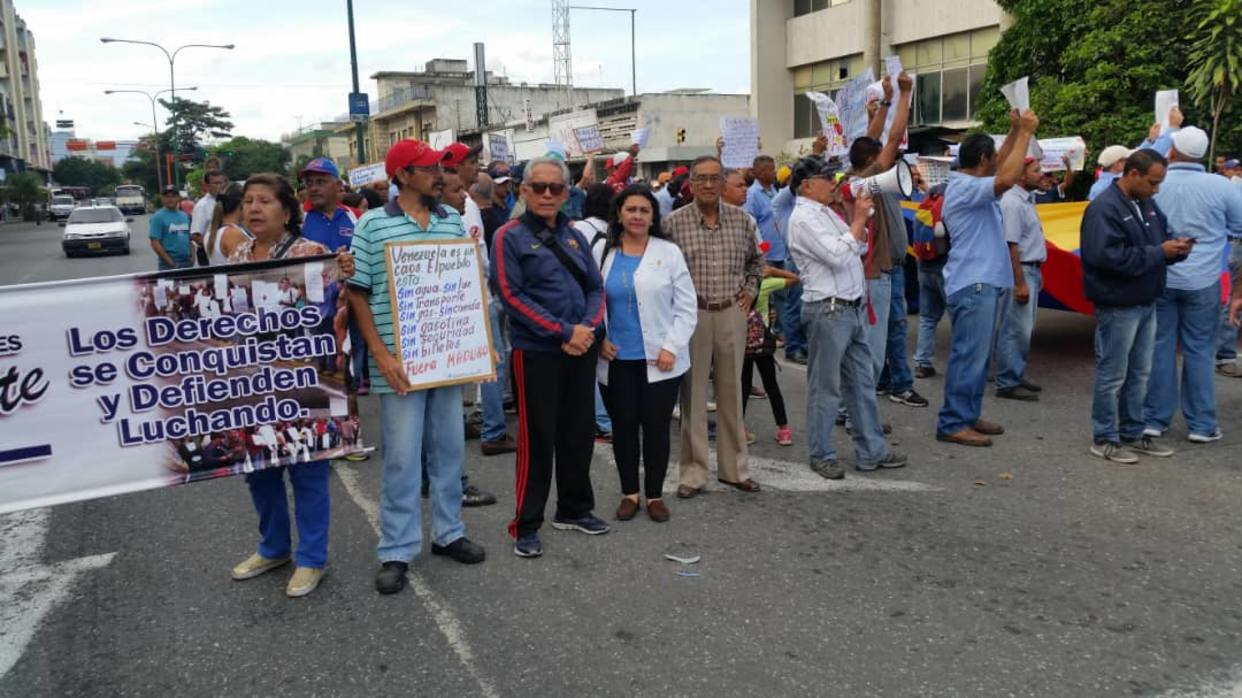
\includegraphics[width=300px]{46.jpg}%
\newline%
%
Habitantes de Barquisimeto, estado Lara, protestan este jueves en reclamo a sus derechos laborales.%
\newline%
%
El periodista Carlos Suárez informó mediante Twitter que la movilización está integrada por sectores gremiales, representantes de ONG y la sociedad civil.%
\newline%
%
Suárez indicó que funcionarios de la policía impiden el paso de los ciudadanos.%
\newline%
%
La concentración inició a las 09:00 am en la avenida Vargas con carrera 24 de la ciudad.%
\newline%
%
Las personas, quienes habían establecido como punto de destino La Plaza Bolívar de la entidad, indicaron que debido a la presencia policial caminarán por la acera de la avenida Vargas hasta llegar a la carrera 18 y de ahí, hasta el punto indicado.%
\newline%
%
\end{document}